\subsection{Explicación del algoritmo implementado}
La heurística golosa que implementamos consiste en buscar el nodo de mayor grado del grafo. A partir de ese nodo v, se construye una clique de frontera máxima de la siguiente manera:

\begin{algorithm}[H]
\caption{Goloso}\label{ej2}
\begin{algorithmic}[1]
\Procedure{Goloso}{$G=(V,E)$}
	\State clique  $\shortleftarrow$ $\{$v nodo de mayor grado$\}$
	\While{ $\{Aumente frontera\}$ }
		\State $\{$Buscar nodo u$\}$ tal que u $\in$ nodos de la frontera y $ d(u) \ge d(p)$ $ \forall p \neq u $ y forme clique con nodos de clique
		\State clique $\cup$ $\{u\}$
	\EndWhile
	\State return |frontera|, |clique|, clique 
\EndProcedure
\end{algorithmic}
\end{algorithm}
Veamos con más detalle ciertos procedimientos para facilitar luego el análisis de complejidad.

Linea 4: Conseguir nodo candidato es básicamente intersecar los adyacentes de cada nodo de la clique que se tiene hasta el momento y luego tomar aquel de mayor grado. ¿Por qué la intersección de los adyacentes?. Porque me aseguro de obtener los nodos de la frontera que sean adyacentes a los nodos de la clique, lo que me permite agrandarla.
¿Por qué el de mayor grado?. Porque será el que mas nodos aporte a la nueva clique del resto de los nodos obtenidos en la intersección.
La intersección entre dos grupos de elementos consiste en recorrer uno de estos grupos y devolver aquellos que tienen coincidencias contra todos los elementos del otro grupo.

Linea 7: Calcular el tamaño de la \textit{frontera} consiste en sumar la cantidad de adyacentes de cada nodo de la clique y restar a este último número resultate las aristas de la clique (que son$ \displaystyle\frac{n(n-1)}{2}$).  

%%%%%%%%%%%%%%%%%%%%%%%%%%%%%%%%%%%%%%%%%%%%%%%%%%%%%%%%%%%%%%%%%%%%%%%%%%%%%%%%%%%%%%%%%%%%%%%%%%%%%%%%%%%%%%%%%%%%%%%%%%%%%%%%%%%%%%%%%%%%%%
%%%%%%%%%%%%%%%%%%%%%%%%%%%%%%%%%%%%%%%%%%%%%%%%%%%%%%%%%%%%%%%%%%%%%%%%%%%%%%%%%%%%%%%%%%%%%%%%%%%%%%%%%%%%%%%%%%%%%%%%%%%%%%%%%%%%%%%%%%%%%%

\subsection{Complejidad}
Veremos la complejidad de la heurística golosa siguiendo paso a paso el algoritmo:
\begin{itemize}
 \item En la linea 2, conseguir el nodo de mayor grado es O(n) pues se recorren todos los nodos.
 \item En la linea 3, se hacen a lo sumo n iteraciones (puede que la clique de frontera máxima sea el grafo entero), luego O(n).
 \item En la linea 4, buscar el nodo candidato tiene una complejidad O($n^{3}$).
\end{itemize}

Luego podemos concluir que la complejidad de la heurística es polinómica (más precisamente O($n^{4}$)). 

Para justificar la complejidad calculada teoricamente utilizaremos el mismo criterio que seguimos con el algoritmo exacto con la única diferencia de que probaremos con grafos más grandes cuya cantidad de nodos va de 1 a 100. A diferencia del algoritmo exacto, la heurísitica presentada puede resolver los casos agregados más rapidamente por ser polinomial.

\begin{figure}[H]
\centering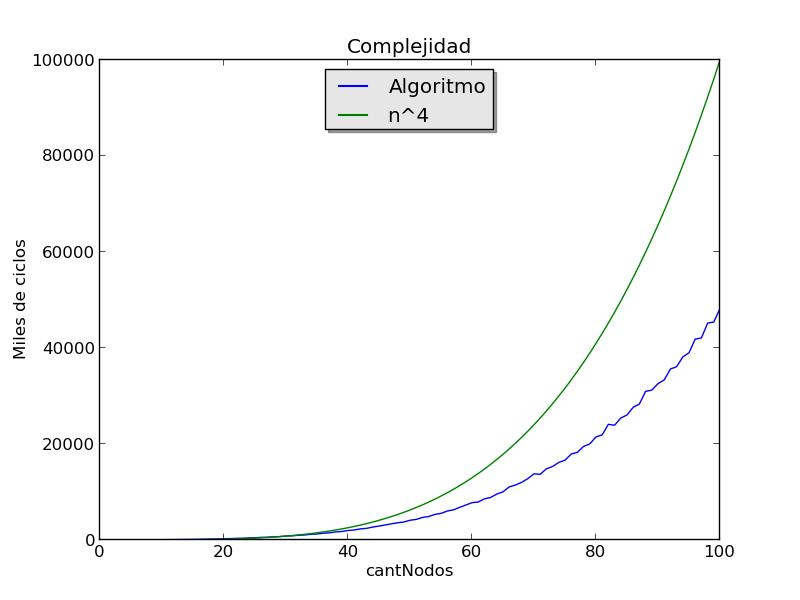
\includegraphics[width=11 cm]{goloso/grafico.jpg}
\caption{Cantidad de ciclos insumidos en función de la cantidad de nodos en el grafo.}
\end{figure}

Podemos observar que el algoritmo se encuentra acotado por $n^4$, cota de complejidad calculada teoricamente.

%%%%%%%%%%%%%%%%%%%%%%%%%%%%%%%%%%%%%%%%%%%%%%%%%%%%%%%%%%%%%%%%%%%%%%%%%%%%%%%%%%%%%%%%%%%%%%%%%%%%%%%%%%%%%%%%%%%%%%%%%%%%%%%%%%%%%%%%%%%%%%
%%%%%%%%%%%%%%%%%%%%%%%%%%%%%%%%%%%%%%%%%%%%%%%%%%%%%%%%%%%%%%%%%%%%%%%%%%%%%%%%%%%%%%%%%%%%%%%%%%%%%%%%%%%%%%%%%%%%%%%%%%%%%%%%%%%%%%%%%%%%%%

\subsection{Casos nefastos}

Los casos en que esta heurística falla, son aquellos en que el nodo de mayor grado del grafo no se encuentra dentro de la clique que se busca o, que a la hora de agrandar la clique buscando el nodo candidato, tome el nodo de mayor grado cuando lo que agrandaba la frontera era uno de menor grado. 
¿Cuán mala puede ser? Tan mala como uno quiera, basta formar, por ejemplo, una estrella con el nodo central de grado máximo y una clique de fontera máxima con tamaño menor al grado máximo. Como ejemplo ilustrativo, mirar la siguiente imagen:

\begin{figure}[H]
\centering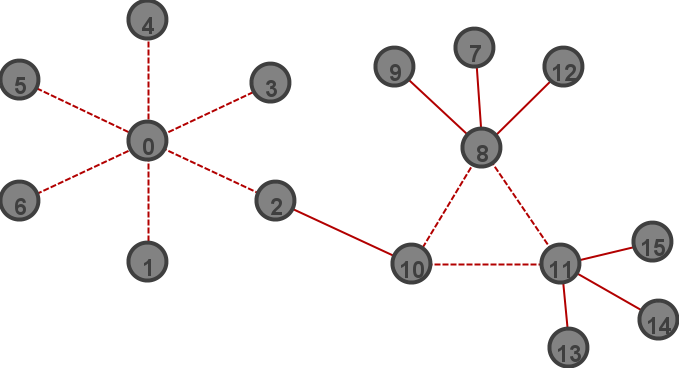
\includegraphics[width=11 cm]{goloso/labl.png}
\caption{Caso 1}
\end{figure}

\begin{center}
    \begin{tabular}{ | l | l | l | l | l | p{5cm} |}
    \hline
    Caso & Frontera exacto & Frontera Goloso & Clique Exacto & Clique Goloso \\ \hline
    1 & 8 & 6 & $\{8,11\}$ & $\{0\}$ \\ \hline
    2 &  &  &  & \\ \hline
    3 &  &  &  & \\
	\hline
    \end{tabular}
\captionof{table}{Frontera devuelta para algoritmo exacto y goloso}
\end{center}
